\chapter{实验设计与结果分析}
\label{chap:chap05}

在本章节,本文介绍了语义关联度的评测数据与评测标准,并在此基础上展开实验,通过与多种基准模型的对比,分别验证了基于WordNet和DBpedia构建的知识关联网络驱动的语义关联度计算模型的性能。

\section{评测标准与实验数据}
\subsection{评测数据}

\begin{table*}[htbp]
    \center
    \smallcaption{MC30: 人为标注的词语间关联度数据示例}
    \vspace{5pt}
    \begin{tabular}{p{2cm}p{2cm}p{1.4cm}p{2cm}p{2cm}p{1.4cm}}
    \hline
    \multicolumn{2}{l}{词对}     & 标注值          & \multicolumn{2}{l}{词对}     & 标注值  \\ \hline
    automobile    &    car    &    3.92 & gem    &    jewel    &    3.84  \\ \hline 
    journey    &    voyage    &    3.84 & boy    &    lad    &    3.76  \\ \hline 
    coast    &    shore    &    3.70 & asylum    &    madhouse    &    3.61  \\ \hline 
    magician    &    wizard    &    3.50 & midday    &    noon    &    3.42  \\ \hline 
    furnace    &    stove    &    3.11 & food    &    fruit    &    3.08  \\ \hline 
    bird    &    cock    &    3.05 & bird    &    crane    &    2.97  \\ \hline 
    implement    &    tool    &    2.95 & brother    &    monk    &    2.82  \\ \hline 
    brother    &    lad    &    1.66 & crane    &    implement    &    1.68  \\ \hline 
    car    &    journey    &    1.16 & monk    &    oracle    &    1.10  \\ \hline 
    cemetery    &    woodland    &    0.95 & food    &    rooster    &    0.89  \\ \hline 
    coast    &    hill    &    0.87 & forest    &    graveyard    &    0.84  \\ \hline 
    shore    &    woodland    &    0.63 & monk    &    slave    &    0.55  \\ \hline 
    coast    &    forest    &    0.42 & lad    &    wizard    &    0.42  \\ \hline 
    cord    &    smile    &    0.13 & glass    &    magician    &    0.11  \\ \hline 
    rooster    &    voyage    &    0.08 & noon    &    string    &    0.08  \\ \hline 
    \end{tabular}
    \label{mc30}
\end{table*}

词语间语义关联度度量是一个十分主观的事情,不同的人基于略有差异的认知,会得到不同的结果。为了方便研究者们的研究,不少语言学家和心理学家提出了很多人工标注的基准数据集~\cite{MC30/Miller02, RG65/RubensteinG65, wordsim353/FinkelsteinGMRSWR02, ws/AgirreAHKPS09, YP130/Yang06verbsimilarity, MEN/BruniTB14},本文列举了以往研究者常用的三种数据集的信息,并且本文利用这三种数据集作为模型的评价数据集合:
\begin{enumerate}
    \item RG65~\cite{RG65/RubensteinG65}:RG65作为经典的数据集,常用来作为语义相似度度量的标准数据集,其中包含有65对英文名词。对于每对词语,受试者们给出一个在$[0,4]$之间的相关度值然后取平均值作为最后的评分,该评分越高,两个词相似度越高,反之亦然。
    \item MC30~\cite{MC30/Miller02}:MC30是RG65中的一个子集,由于时间的迁移,RG65中一些词的相关性发生了变化,研究者重新评分其部分子集来构成了MC30,如表格~\ref{mc30}所示,本文给出了其全部示例。
    \item WS353~\cite{wordsim353/FinkelsteinGMRSWR02}:WS353中包含353对英文单词,其词性包含名词、动词以及形容词,是常用的词语间语义关联度度量的评测数据。词对间关联度评分取值范围为$[0,10]$,值越大,两个单词关联度越高。
\end{enumerate}
最后在表格~\ref{golden},本文整理并给出本文所使用的评测数据集及其简要信息。

\begin{table}[htbp]
    \center
    \smallcaption{词语间语义关联度评测数据集}
    \vspace{5pt}
    \begin{tabular}{|p{1.8cm}|p{1.8cm}|p{1.8cm}|p{5cm}|}
    \hline
    数据名称    & 词对数量    & 取值范围      & 引文 \\ \hline
    RG        & 65         & [0,4]       & Rubenstein\&Goodenough1965       \\ \hline
    MC        & 30         & [0,4]       & Miller\&Charles1991          \\ \hline 
    WS353     & 353        & [0,10]      & Finkelstein et al.2002         \\ \hline
    \end{tabular}
    \label{golden}
\end{table}

\subsection{评测标准}
不同评测数据集的关联度标注值取值范围不同,无法通过简单的距离计算来衡量模型表现。同之前的语义关联度计算研究一样,本文采用模型估计值与评测数据标准值之间的相关系数来衡量模型表现。两组变量的相关系数反映了两组变量之间在统计关系上的相关程度,其取值范围一般是$[-1, 1]$,取值越大相关程度越高,其中-1表示两组变量负相关,1则表示正相关。下面给出了本文中使用的三种相关系数及其简要介绍:

\begin{enumerate}
    \item 皮尔森(Pearson)相关系数:本文被记为$\gamma$,反映了两组变量之间的线性相关程度,当一组变量的变化与另一组变量的变化成比例相关时,这两个变量具有线性关系。其计算公式如下:
    \begin{equation}
        \label{pearson}
        \gamma(X, Y) = \frac{E[(X-\mu_X)(Y-\mu_Y)]}{\sigma_X \sigma_Y}
    \end{equation}
    \noindent 其中分子部分构成了$X$和$Y$的协方差,$E(\cdot)$表示求一组变量的期望值,$\mu_X$和$\mu_Y$分别表示两组变量$X$和$Y$的平均值,$\sigma_X$和$\sigma_Y$则分别表示两组变量的标准差。
    \item 斯皮尔曼秩(Spearman's rank)相关系数:本文被记为$\rho$,反映了两组变量的移动方向是否一致。斯皮尔曼秩相关系数检验的不是数据之间的关系,而是数据排名之间的关系,这对于数据异常值和数据规模具有更强的鲁棒性。其计算过程往往需要先对原始数据排序,对于两组原始变量$X$和$Y$,排序后得到$rg_X$和$rg_Y$,然后通过下面的公式来计算其相关系数值:
    \begin{equation}
        \label{spearman}
        \rho(X, Y) = \gamma(rg_X, rg_Y) =  \frac{E[(rg_X-\mu_{rg_X})(rg_Y-\mu_{rg_Y})]}{\sigma_{rg_X} \sigma_{rg_Y}}
    \end{equation}
    \noindent 其中符号含义类比公式~\ref{pearson}。可见,当两组变量排序前后相对顺序一致时,斯皮尔曼秩相关系数等于皮尔森相关系数。
    \item 皮尔森相关系数与斯皮尔曼秩相关系数的调和平均(Harmonic mean)相关系数:这部分本文取皮尔森相关系数与斯皮尔曼秩相关系数的调和平均值作为最后的评价指标,公式如下。
    \begin{equation}
        \label{harmonic}
        \mu(X, Y) = \frac{2\gamma(X, Y)\rho(X, Y)}{\gamma(X, Y)+\rho(X, Y)}
    \end{equation}
\end{enumerate}

\subsection{实验数据}

\textbf{基于WordNet构建的知识关联网络:}
基于WordNet构建知识关联网络时,本文采用的版本是WordNet 3.1。本文首先遍历其中所有同义词集即实体,抽取出每个实体周围的三种关系:上位关系(hypernyms)、下位关系(hyponyms)以及部分整体关系(member holonyms),组成知识关联网络中实体层之间的关系,其中节点与边规模如表格~\ref{wordnet_data}~所示。由表中数据可见实体之间的关系比较稀疏。

\begin{table}[htbp]
    \center
    \smallcaption{WordNet实体及其边规模信息}
    \vspace{5pt}
    \begin{tabular}{|p{1.6cm}|p{1.6cm}|p{1.6cm}|p{2.5cm}|p{1.6cm}|}
    \hline
    实体   & 上位关系 & 下位关系 & 部分整体关系 & 边总数   \\ \hline
    117,660   & 89,090 & 89,090 & 12,294 & 190,474    \\ \hline
    \end{tabular}
    \label{wordnet_data}
\end{table}

\textbf{基于DBpedia构建的知识关联网络:}
基于DBpedia构建知识关联网络的过程中,要通过Wikipedia页面信息建立起词语与实体之间的关系。本文采用维基百科2016年10月份的备份数据\footnote{https://dumps.wikimedia.your.org/},并通过简单的文本分析建立起词语与维基百科之间的联系,然后再通过文章独有的数字ID建立起与DBpedia中实体之间的关系。其中Wikipedia与DBpedia的实体规模信息如表格~\ref{wiki_data}~所示。

之前本文提到Wikipedia中的实体与DBpedia中一一对应,表格~\ref{wiki_data}~中所示DBpedia中的实体数量要多于Wikipedia中页面所描述的实体数。这是因为DBpedia不仅仅包含了从Wikipedia中抽取的实体,也连接了其他语义信息库如原语库、YAGO知识图谱等等。
在连接Wikipedia页面与词语时,本文首先要对Wikipedia的语料库做简单的预处理。本文移除了文本中的停用词与标点符号,忽略了其中包含单词数少于50的页面,同时对于其中一些用处较少的命名空间(namespace)如分类(Category)、文件(File)以及模板(Template),\footnote{https://en.wikipedia.org/wiki/Wikipedia:Namespace}本文不予考虑。

% \renewcommand\arraystretch{1.2}
\begin{table}[htbp]
    \center
    \smallcaption{Wikipedia和DBPedia信息}
    \vspace{5pt}
    \begin{tabular}{|p{2cm}|p{2cm}|p{2cm}|p{2cm}|}
    \hline
              & 实体数    & 日期        \\ \hline
    Wikipedia & 5.5M     & 2016-10     \\ \hline
    DBPedia   & 6.6M     & 2016-10     \\ \hline
    \end{tabular}
    \label{wiki_data}
\end{table}


\section{知识关联网络驱动的语义关联度计算模型评估}
在此节中,本文分别给出基于WordNet和DBpedia构建的知识关联网络中遇到的模型参数设置,以及模型在标准评测数据集上的表现。

\subsection{基于WordNet构建的知识关联网络}
\textbf{参数设置:}
在基于WordNet构建的知识关联网络中,本文基于自注意力机制学习到实体的向量表示,其中模型的参数设置如下:
\begin{itemize}
    \item 在实体层,本文采用两层的自注意力模型来训练实体向量表示。第一层的输入为WordNet中实体所对应的词向量的平均值,输出维度为256,多头注意力值$K=4$,采用拼接的方式组合学习到的4个实体向量表示。而第二层输出维度256,$K=4$,然后取4个实体向量的平均值,作为最后的实体向量表示输出。
    \item 训练自注意力模型时,本文采用Adam算法来优化目标函数,其中初始学习率设置为0.01,权重衰减值(weight\_decay)设置为0。
\end{itemize}


\begin{table*}[htbp]
    \center
    \smallcaption{不同网络嵌入模型在实体层语义关联度计算上的相关系数表现:皮尔森-$\lambda$, 斯皮尔曼秩-$\rho$, 调和平均-$\mu$相关系数}
    \vspace{5pt}
    \begin{tabular}{l|c|c|c|c|c|c|c|c|c|c}
    \hline
    \multirow{2}{*}{图嵌入模型}     & \multirow{2}{*}{策略} & \multicolumn{3}{c|}{$\lambda$} & \multicolumn{3}{c|}{$\rho$} & \multicolumn{3}{c}{$\mu$} \\ \cline{3-11} 
     &
       &
      \multicolumn{1}{c|}{\textbf{MC}} &
      \multicolumn{1}{c|}{\textbf{RG}} &
      \multicolumn{1}{c|}{\textbf{WS}} &
      \multicolumn{1}{c|}{\textbf{MC}} &
      \multicolumn{1}{c|}{\textbf{RG}} &
      \multicolumn{1}{c|}{\textbf{WS}} &
      \multicolumn{1}{c|}{\textbf{MC}} &
      \multicolumn{1}{c|}{\textbf{RG}} &
      \multicolumn{1}{c}{\textbf{WS}} \\ \hline
    \multirow{2}{*}{node2vec} &
      max &
      \multicolumn{1}{c|}{0.535} &
      \multicolumn{1}{c|}{0.618} &
      \multicolumn{1}{c|}{-0.049} &
      \multicolumn{1}{c|}{0.344} &
      \multicolumn{1}{c|}{0.461} &
      \multicolumn{1}{c|}{-0.093} &
      \multicolumn{1}{c|}{0.419} &
      \multicolumn{1}{c|}{0.528} &
      \multicolumn{1}{c}{-0.064} \\ \cline{2-11} 
                               & mean & 0.142 & 0.263 & -0.001 & 0.197 & 0.320 & -0.039 & 0.165 & 0.289 & -0.002 \\ \hline
    \multirow{2}{*}{GraphSage} & max  & 0.872 & 0.808 & 0.421 & 0.833 & 0.799 & 0.173 & 0.852 & 0.803 & 0.245 \\ \cline{2-11} 
                               & mean & 0.706 & 0.637 & 0.464 & 0.661 & 0.641 & 0.458 & 0.683  & 0.639 & 0.461 \\ \hline
    \multirow{2}{*}{Un-GAT}       & max  & $\bf 0.913$ & $\bf 0.848$ & 0.435 & $\bf 0.845$ & $\bf 0.816$ & 0.397 & $\bf 0.878$  & $\bf 0.832$ & 0.415 \\ \cline{2-11} 
                               & mean & 0.632 & 0.662 & $\bf 0.549$ & 0.635 & 0.652 & $\bf 0.515$ & 0.633 & 0.657 & $\bf 0.531$ \\ \hline
    \end{tabular}
    \label{table5-5}
\end{table*}


\textbf{模型表现:}
WordNet中存储了描述词语不同含义的同义实体集,这些实体之间的相关程度可以反映不同单词之间的关联性。回顾章节\ref{chap:chap03}中描述的基于WordNet构建的知识关联网络,其表现为有向无权图。为了丰富词语层的关联程度,本文在图注意力网络(GAT)的基础上,采用无监督训练的方式训练得到实体向量表示。在表格~\ref{table5-5}~中,本文基于三种基准评测数据集,给出了三种网络嵌入模型在实体层之间的关联程度$F_e(w_i, w_j)$(见前文公式~\ref{F_e}~)上的相关系数表现。其中$max$和$mean$分别对应于章节\ref{chap:chap03}中提到的计算实体层语义关联度的两种策略,对比模型的参数设置如下:
\begin{itemize}
    \item 其中node2vec~\cite{kdd/GroverL16}是一种基于随机游走的无监督图嵌入模型,对于其提出的偏置随机游走策略,本文在公式~\ref{zeta}~中有过详细介绍。在本章节的对比实验中,本文设置其中的两个参数$p$和$q$均为1,游走长度为50,邻居窗口大小为10,对每个节点随机游走其相关序列采样10次。优化器采用Adam,其中学习率设置为0.01,权重衰减设置为0.0005。模型输出实体向量维度设置为256。
    \item 而GraphSage~\cite{nips/HamiltonYL17}是一种基于神经网络的图嵌入模型,这种模型通过不同的聚合算子来综合考虑固定邻居特征对当前节点的影响。本文采用基于平均策略的两层的GraphSage来进行实验,第一层和第二层的向量输出维度均设置为256,其中对于每个节点,其邻居采样大小设置为5。模型优化器设置为Adam,其中学习率为0.01,权重衰减值为0。
\end{itemize}

基于上述模型参数设置,从表格~\ref{table5-5}~中可以看出,基于$max$的策略取实体集之间的最大关联度作为计算结果,要比取平均值的$mean$策略效果要好很多。这在一定程度上也符合人类判断直觉,当两个词的某个意思关联度比较高而其他含义相关度不高时,人们常常人为两个词是相关的。此外,从表格~\ref{table5-5}~中还可以看出,基于图注意力网络的无监督训练得到结果取得了最好的效果,即可以更好地表征实体的语义特征。接下来本文将介绍基于图注意力网络的无监督训练与词语层关联度度量对最终结果的影响。

\begin{figure}[htbp]
    \begin{minipage}{0.48\textwidth}
      \centering
      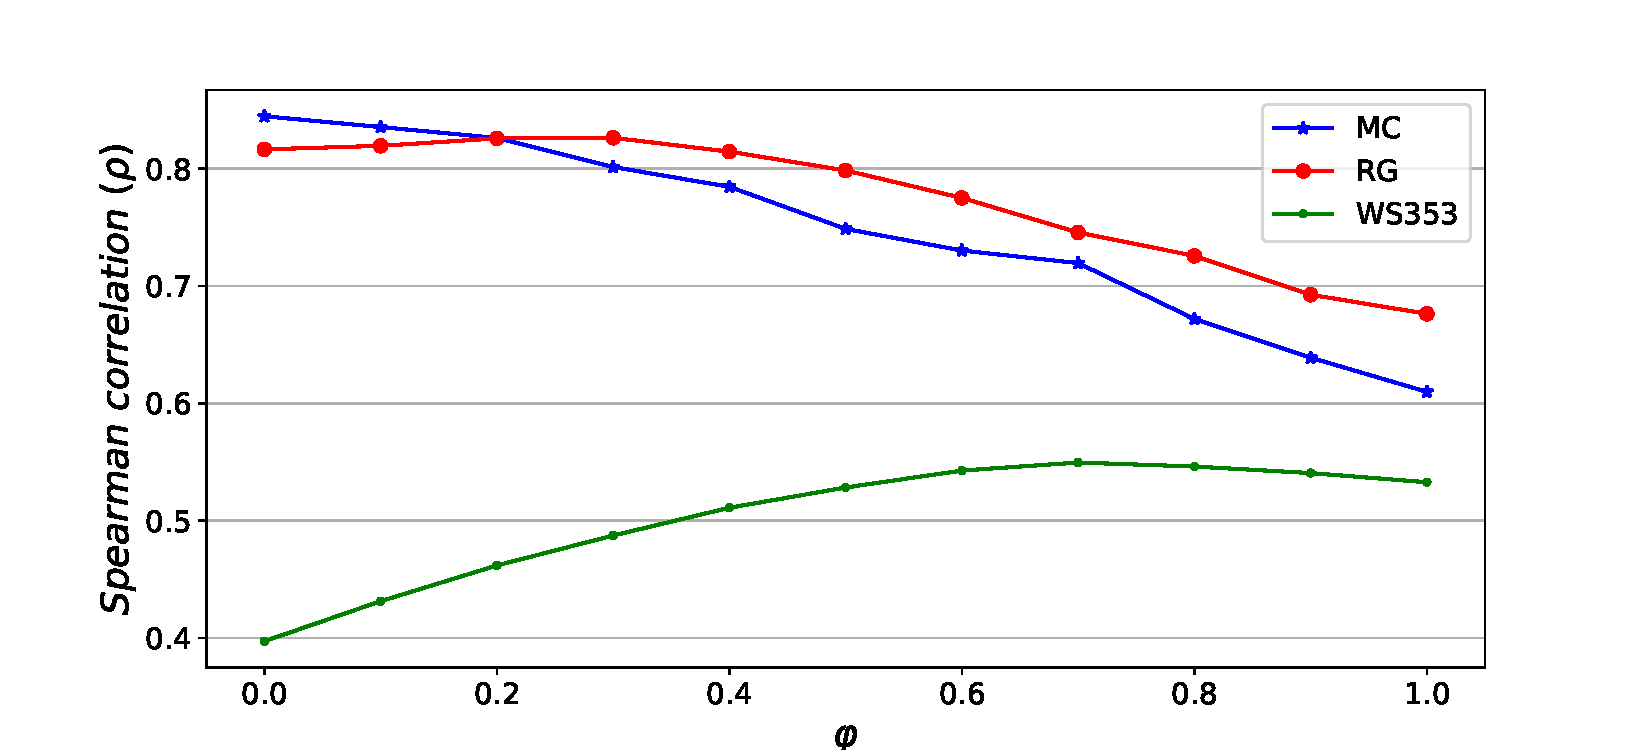
\includegraphics[width=1\textwidth]{params_lambda_w_max.pdf}
      \smallcaption{基于max策略的语义关联度计算中$\lambda$参数对于模型表现的影响}
      \label{fig:lambda_w_max}
    \end{minipage}\hfill
    \begin{minipage}{0.48\textwidth}
      \centering
      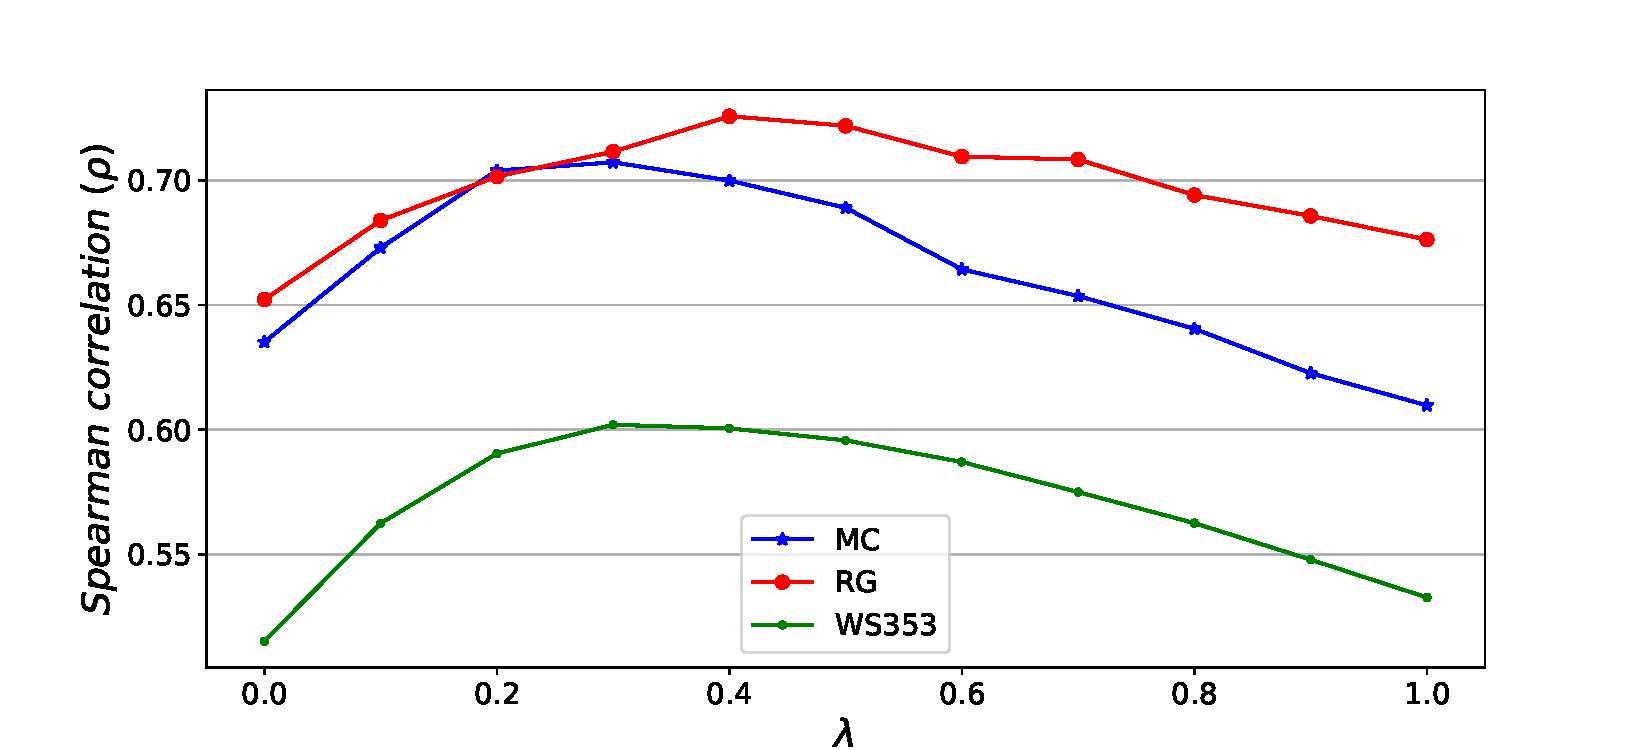
\includegraphics[width=1\textwidth]{params_lambda_w_mean.pdf}
      \smallcaption{基于mean策略的语义关联度计算中$\lambda$参数对于模型表现的影响}
      \label{fig:lambda_w_mean}
    \end{minipage}
    \label{fig:wordnet_sr}
\end{figure}

前文提到的参数$\varphi$用来权衡词语层层关联度与实体层关联度对最终语义关联度的影响,如图\ref{fig:lambda_w_max}和图\ref{fig:lambda_w_mean},基于自注意力机制的网络嵌入下的不同实体层关联度方式,本文给出了$\varphi$对最终结果的影响。从图\ref{fig:lambda_w_max}可以看出在基于max策略的实体层关联度度量模型中,对于MC和RG这两个数据集,$\varphi$取$0$时的效果最好。这是因为本文在网络输入初始化的时候,采用的是实体相关联的词向量平均值作为输入,这在一定程度上已经考虑了从文本中训练得到的语义向量信息,而WordNet知识关联网络嵌入则起到了学习词语背后相关联实体的语义内容的作用,可以看出最后结果要比单纯文本训练词向量的结果要好。而对于WS这个数据集,当$\varphi$取$0.8$时,模型效果最优,词语层关联度起主要贡献。另外在图\ref{fig:lambda_w_mean}基于mean策略的中,知识关联网络嵌入中学习到的实体语义信息被平均弱化,表现不如基于max的策略。但是当$\varphi$取$0.3$的时候,网络嵌入学习得到的语义信息还是可以为词向量补充语义信息。

\subsection{基于DBpedia构建的知识关联网络}
\textbf{参数设置:}
在基于DBpedia构建的知识关联网络中,需要确定的模型参数如下:
\begin{itemize}
    \item 在~\ref{dbpedia_word2vec}~中,本文在处理后的Wikipedia语料库上训练Word2Vec模型,在这部分,本文采用\emph{100维向量输出, 30窗口大小以及Skip-gram model与negative sampling}的结合来训练得到词向量。
    \item 在实体层属性空间嵌入部分,本文设置 \emph{间隔margin $\ell=0.05$, 输出维度 $d=100$, 负采样数 $k=50$}, 本文还设置随机梯度下降的学习率为$0.01$来优化Margin Ranking损失。
    \item 在实体层网络拓扑结构空间嵌入部分,本文采用Skip-gram模型来训练随机采样的序列,其中偏置随机游走中$p$和$q$的值分别设置为0.7和0.3,同时本文采用\emph{100维的输出维度, 10的窗口大小}来训练模型。
\end{itemize}


\begin{table*}[htbp]
    \center
    \smallcaption{不同的权重分配策略构建的知识关联网络在三种数据集上的皮尔森-$\lambda$, 斯皮尔曼秩-$\rho$, 调和平均-$\mu$相关系数}
    \vspace{5pt}
    \begin{tabular}{l|c|c|c|c|c|c|c|c|c}
    \hline
    \multirow{2}{*}{模型} & \multicolumn{3}{c|}{$\lambda$}     & \multicolumn{3}{c|}{$\rho$}          & \multicolumn{3}{c}{$\mu$} \\ \cline{2-10} 
                           & \textbf{MC}&\textbf{RG}&\textbf{WS} & \textbf{MC}&\textbf{RG}&\textbf{WS} & \textbf{MC}&\textbf{RG}&\textbf{WS}\\ \hline
    $KAN_{cnt}$            & 0.850 & 0.826 & 0.630 & 0.836 & 0.805 & 0.633 & 0.842 & 0.816 & 0.631   \\ \hline
    $KAN_{tf\_idf}$        & $\bf 0.892$  & $\bf 0.887$ & $\bf 0.783$ & $\bf 0.866$ & $\bf 0.861$ & $\bf 0.835$ & $\bf 0.879$ & $\bf 0.874$ & $\bf 0.808$ \\ \hline
    \end{tabular}
    \label{table5-6}
\end{table*}


\textbf{模型表现:}
回顾实体层之间的关联度度量那节,对于实体所处的拓扑结构空间,本文采用两种策略来为实体之间的关系分配权重:1)$W_{cnt}(e_i,e_j)$表示实体$e_i$与实体$e_j$对应的锚文本之间的共现频率;2)$W_{tf\_idf}(e_i,e_j)$评估了实体$e_j$的锚文本相对于$e_i$所对应文章的重要程度。基于这两种评价策略,本文分别构造得到两种知识关联网络$KAN_{cnt}$以及$KAN_{tf\_idf}$。从表格~\ref{table5-6}~中可以看出,基于$KAN_{tf\_idf}$的语义关联度度量模型在不同评测数据集上表现都更加好。这是因为$TF-IDF$适当的调节了文章中的关键词词频,通过考虑逆文档频率降低了高频通用词的权重,使得词语与文档之间的关联度度量更准确。

前文提到的参数$\alpha$用来平衡属性空间关联度与拓扑结构空间关联度之间的权重。为了得到最优的模型表现和提高模型鲁棒性,本文不在最终评测数据集上调节参数,而是选择在数据集\emph{WS-Rel}~\cite{ws/AgirreAHKPS09}试验参数$\alpha$对最终结果的影响。\emph{WS-Rel}中包含有252个单词对以及关联度评分值,这个数据集在很多关联度数据集中没有被使用。图~\ref{fig:alpha}~展示来不同的$\alpha$取值对最后Spearman相关系数($\rho$)的影响,可以看出当$\alpha$趋近于0.5的时候,$\rho$取值最大,这意味着属性空间的语义信息与拓扑结构中所包含的隐含语义信息对语义关联度的计算有着相同的共现。

另一个参数$\varphi$起到权衡知识关联网络中实体层$F_e$与词语层语义关联度$F_w$的作用。图~\ref{fig:lambda}~展示了$F_e$和$F_w$对在最终评测数据集上对最终语义关联度计算的影响,可见当$\varphi=0.2$时,Spearman相关系数$\rho$取值达到最大。显然,$F_w$对最后的语义关联度计算影响更大,起到了主导的作用,而$F_e$中包含的隐含语义信息也有效的丰富了词语的语义空间,使得最终的关联度计算值有所提升。

\begin{figure}[htbp]
    \begin{minipage}{0.48\textwidth}
      \centering
      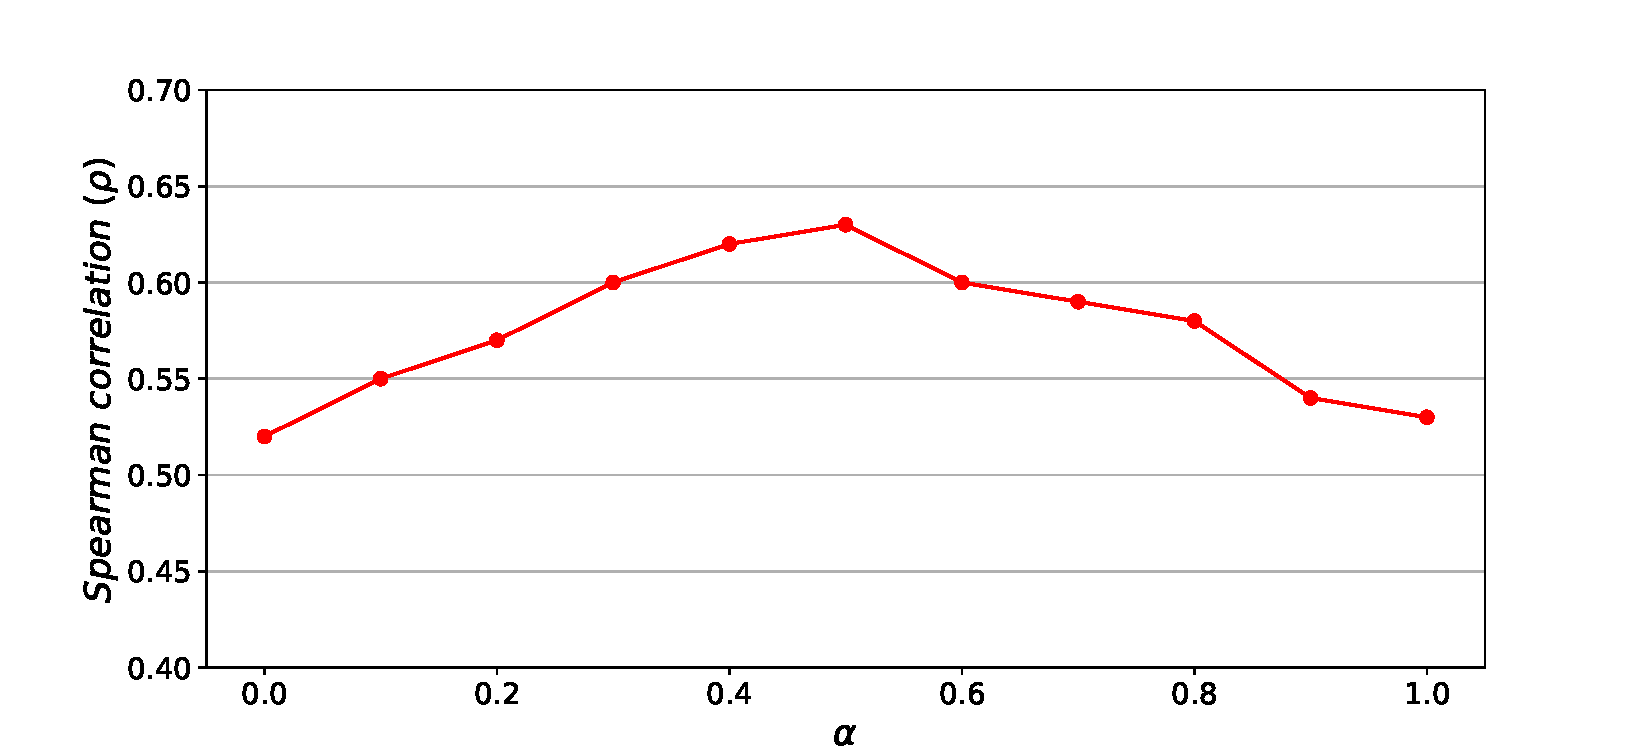
\includegraphics[width=1\textwidth]{params_alpha.pdf}
      \smallcaption{$\alpha$对实体层之间关联度的影响}
      \label{fig:alpha}
    \end{minipage}\hfill
    \begin{minipage}{0.48\textwidth}
      \centering
      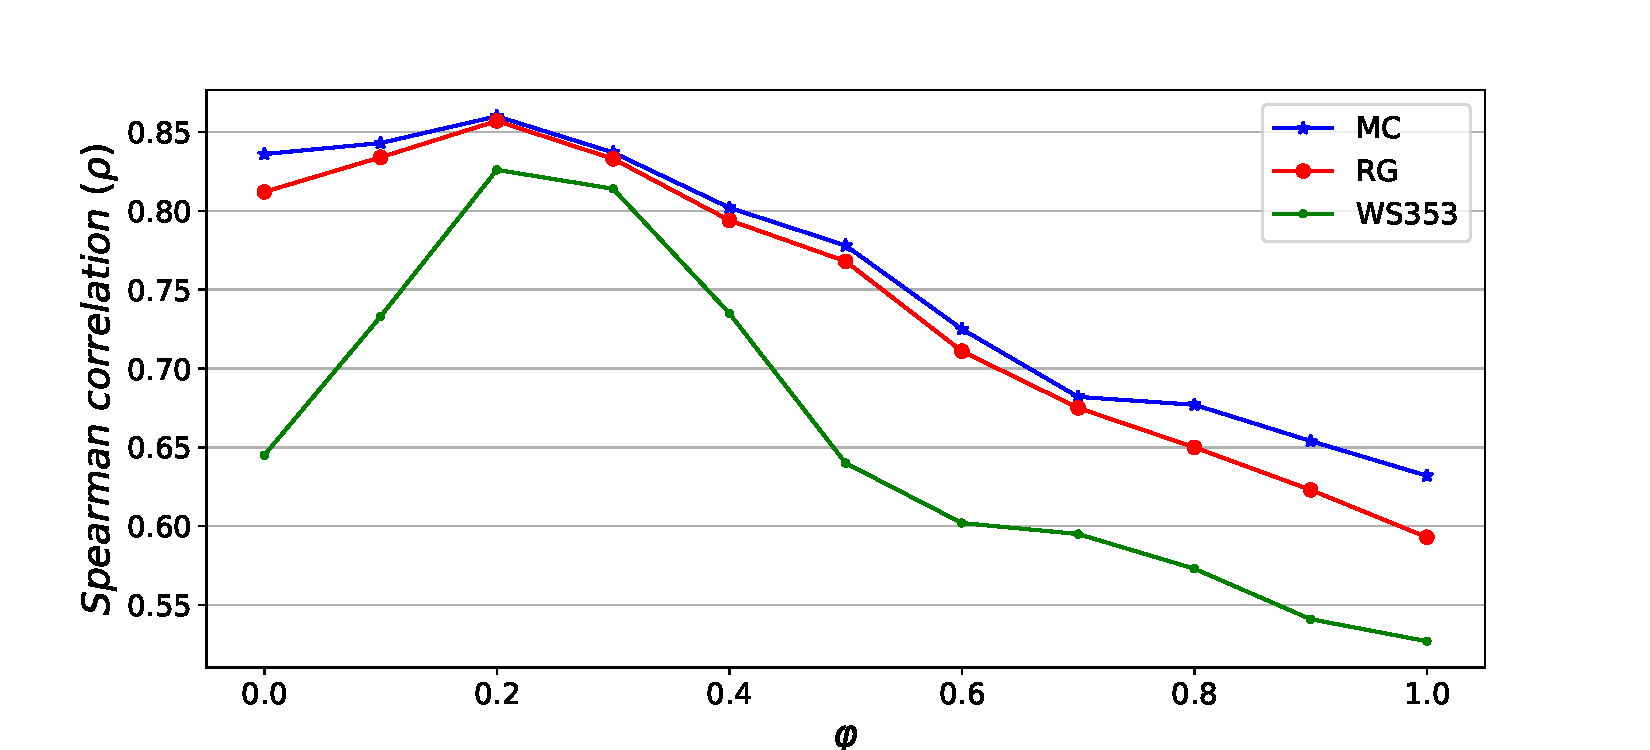
\includegraphics[width=1\textwidth]{params_lambda_d.pdf}
      \smallcaption{$\lambda$参数对于模型表现的影响}
      \label{fig:lambda}
    \end{minipage}
\end{figure}


\section{模型的对比与分析}
此节基于表格\ref{golden}中提到的三种人为标注的高质量语义关联度数据,对比了传统语义关联度计算模型与本文提出的知识关联网络驱动的计算模型之间的差异,并分析了多种模型之间的差异。

\textbf{对比模型:}
基于标准评估数据,本文主要对比了以下几种语义关联度计算模型论文中的报告结果:
\begin{itemize}
    \item 基于共现原则的方法:ESA\cite{aaai/StrubeP06}中则采用$tf-idf$技术来为文本中的词语分配权重,然后利用词语对应的文本中包含的词语$tf-idf$权重向量来计算语义关联度;SSA\cite{aaai/HassanM11}中利用维基百科中词语上下文中的实体信息为词语构建语义画像,然后通过基于规则的方法计算词语间关联度;Word2Vec\cite{corr/Mikolov13}利用词语之间的共现信息来将词语表征在向量空间,由此来计算语义关联度;SaSA\cite{aaai/WuG15}利用维基百科中词语对应的不同实体,在词义层面学习得到词语向量表示,解决了Word2Vec中无法表征词语多义性的缺点。
    \item 基于关联网络的方法:AN\cite{aaai/ZhangZH15}和HAN\cite{aaai/GongXH18}提出关联网络的概念来连接起词语与知识库实体之间的关系,然后综合考察了词语层与实体层的语义关联度。
\end{itemize}

本文中提出的模型中被作为对比的是:
\begin{itemize}
    \item 基于WordNet构建的知识关联网路驱动的语义关联度计算:在这部分实体层向量学习中,采用基于网络注意力机制的方法取得了较好的结果,这里记基于这种机制的语义计算模型为$WordNet\_KAN_{gat}$,取$\varphi=0$的结果作为对比结果。
    \item 基于DBpedia构建的知识关联网路驱动的语义关联度计算:这部分中,基于$tf-idf$的实体层网络取得了最优的结果,我们记基于这种方法的语义计算模型为$DBpedia\_KAN_{tf\_idf}$,取$\varphi=0.2$的结果作为对比结果。
\end{itemize}


\begin{table*}[htbp]
    \center
    \smallcaption{不同语义关联度计算模型在三种数据集上的皮尔森-$\lambda$, 斯皮尔曼秩-$\rho$, 调和平均-$\mu$相关系数}
    \vspace{5pt}
    \begin{tabular}{l|c|c|c|c|c|c|c|c|c}
    \hline
    \multirow{2}{*}{模型} & \multicolumn{3}{c|}{$\lambda$}     & \multicolumn{3}{c|}{$\rho$}          & \multicolumn{3}{c}{$\mu$} \\ \cline{2-10} 
                           & \textbf{MC}&\textbf{RG}&\textbf{WS} & \textbf{MC}&\textbf{RG}&\textbf{WS} & \textbf{MC}&\textbf{RG}&\textbf{WS}\\ \hline
    ESA                    & 0.588 &  - -  & 0.503 & 0.727 &  - -  & 0.748 & 0.650 &  - - & 0.602    \\ \hline
    SSA                    & 0.879 & 0.861 & 0.590 & 0.843 & 0.833 & 0.604 & 0.861 & 0.847 & 0.597   \\ \hline
    Word2Vec               & 0.852 & 0.834 & 0.633 & 0.836 & 0.812 & 0.645 & 0.844 & 0.823 & 0.639   \\ \hline
    SaSA                   & 0.886 & 0.882 & 0.733 & 0.855 & 0.851 & 0.739 & 0.870 & 0.866 & 0.736   \\ \hline
    $AN_{wiki}$            & 0.865 & 0.858 & 0.740 & 0.848 & 0.843 & 0.813 & 0.856 & 0.850 & 0.775   \\ \hline
    $HAN_{wiki}$           & 0.886 & 0.884 & 0.772 & 0.860 & 0.857 & 0.826 & 0.873 & 0.870 & 0.798   \\ \hline
    $WordNet\_KAN_{gat}$   & $\bf 0.913$ & 0.848 & 0.435 & 0.845 & 0.816 & 0.397 & 0.878  & 0.823 & 0.570 \\ \hline
    $DBpedia\_KAN_{tf\_idf}$        & 0.892 & $\bf 0.887$ & $\bf 0.783$ & $\bf 0.866$ & $\bf 0.861$ & $\bf 0.835$ & $\bf 0.879$ & $\bf 0.874$ & $\bf 0.808$ \\ \hline
    \end{tabular}
    \label{table5-7}
\end{table*}

\textbf{模型表现的对比与分析:}
表格~\ref{table5-7}~给出了本文提出的两种模型以及多种对比模型在MC30、RG65以及WS353三种数据集上的相关系数表现。
从表格中可以看出,传统基于关联网络的方法$AN_{wiki}$和$HAN_{wiki}$通过关联词语与语料库文档的关系,更好地捕捉到了词语的语义特征,改善了传统基于共现的方法的缺点。本文提出的模型中,基于WordNet的语义关联度计算模型$WordNet\_KAN_{gat}$仅在MC30数据集上的表现优于$AN_{wiki}$和$HAN_{wiki}$,这是因为WordNet中仅仅存储了实体之间的相对关系与位置信息,相对于文本库中抽取得到的手工特征显得表现力不足。而基于DBpedia的语义关联度计算模型$DBpedia\_KAN_{tf\_idf}$弥补了这个缺点,更好地同时考虑了实体所处的属性空间与拓扑结构空间,向量化的表示也使本文的模型更加灵活,更具表达力。


\section{本章小结}
实验部分,本章基于传统评测数据,对测评标准进行了介绍。对于基于WordNet构建的知识关联网络,本章对比了多种网络嵌入模型的表现,验证了基于自注意力机制的无监督网络嵌入模型的效果。对于基于DBpedia构建的知识关联网络,本章对比了实体层实体属性空间与拓扑空间语义信息对最后关联度度量结果的影响。最后通过与传统基准模型的对比,验证了本文提出的模型的效果。
